\documentclass[a4paper, 12pt]{article}
\usepackage[a4paper,textwidth=170mm,textheight=245mm]{geometry}

\usepackage[utf8]{inputenc}
\usepackage{todonotes}
\usepackage{amsmath}
\usepackage{parskip}
\usepackage{listings}
\usepackage{float}
\usepackage{url}
\usepackage{hyperref}

% For the wrapfigure
\usepackage{wrapfig}
\usepackage{caption}
\usepackage{subcaption}
\usepackage{color, colortbl}

\definecolor{Green}{rgb}{0.3,0.85,0.24}

\begin{document}
\date{January 2018}

\title{\Large Classy: Feature Evaluation using Naive Bayes for Genre Classification}

\author{
{Michael Sörsäter}\\
IDA Linköping
}

\maketitle

\subsection*{Abstract}

What defines a genre?
What are the key elements that characterizes rap, pop and electronic music?
In this project a corpus was created, including 6 genres and 3000+ tracks.
Naive Bayes was used to classify the genres.
A feature analysis and evaluation was made to identify \textit{good} features when classifying the lyrics.

\section{Introduction}
Music is a big part of our modern society.
According to Spotify, I listened to over 60 000 minutes of music during 2017. \cite{spotify}
As everything else in our world we order things and place them in different categories.

Music is often categorized in large genres like \textit{pop}, \textit{rap} and \textit{rock}, which is categorized further, like \textit{indiepop}, \textit{dream pop} and \textit{synth pop}.
The most defining features of a genre is the sound, instruments used, the tempo and the structure of the track, like number of verses and choruses.
Even if this may have the greatest impact when deciding the genre, the lyrics tend to follow certain patterns.

I think that pop music generally tend to be about love and easier subjects whereas rap usually have a more complex language and a storytelling structure.

In this project a classifier was implemented to determine the genres of tracks.
Different features were considered and evaluated, when classifying the genres, to see if they improved the accuracy.
Focus lied on comparing the two genres pop and rock but also all 6 genres.

\pagebreak
\section{Theory}
The Naive Bayes classifier is commonly used for music classification and have shown in previous work to be an effective model for document classification. \cite{Canicatti} \cite{optimality} \cite{bou2012classifying}

\subsection{Naive Bayes}
Naive Bayes build a probabilistic model that uses arbitrary features from documents.
When training the model features are extracted from different documents and are given to the model together with the document class.
For each feature and class the probability in formula \ref{eq:feat} is calculated where $ feat_{i}$ is feature i and $ class_k $ is class k.

\large
\begin{equation}
    p (feat_{i}|class_{k})
    \label{eq:feat}
\end{equation}
\normalsize

When predicting the class of a document the same features are extracted and given to formula \ref{eq:bayes} where there exist $K$ classes and $n$ features for each document.
The probability of the class is multiplied by all features explained in formula \ref{eq:feat}.
The predicted class k is the k that maximizes the expression.

\large
\begin{equation}
    \hat{y} = \underset{k \in \{1,2,...,K\}}{argmax} \, \, \, p(class_{k}) \prod_{i=1}^{n} p (feat_{i}|class_{k}
    \label{eq:bayes}
\end{equation}
\normalsize

The strength of the Naive Bayes classifier is that the features are arbitrary.
The model determine the importance for all features and let informative features influence the prediction as well as assign uninformative features with low probabilities. \cite{tm-lecture} \cite{rish2001empirical}

\section{Data set}
\label{sec:dataset}
The acquisition of a good data set is a task that requires careful consideration.
Usually one artist (will use the word artist for artist/band/group) is labeled with just one genre and all tracks produced by that artist are assumed to be that genre.
This assumption can result in bad classification as one artist is not bound to one genre.
Previous obtained data sets were considered.
The problem with copyrighted lyrics, often have the impact that bag of words models are used where the different words are converted to integers. \cite{million}
This representation makes it hard to work with the models and to evaluate the result, features like n-grams and structure of tracks is impossible to use.
Many data sets found have not been classified with genres or had to many genre classes in them.
For these reasons I decided to create my own corpus.

When the data set was created three steps were followed.
Firstly, getting lists of tracks tagged with their genre.
Secondly, from the name of the tracks, get an URL to a webpage hosting lyrics.
Thirdly, from the URLs, scrape and store the lyrics.

\subsection{List of tracks}
The following criterions were considered when looking for lists of tracks:
\begin{itemize}
    \item {\textbf{Organization} - Lists made by individuals can be subjective and is therefore avoided.
    Lists by organizations tend to be more thought through.}
    \item {\textbf{Reliable} - The producer behind the list should have a lot of experience and knowledge about music.}
    \item {\textbf{Genre cover} - The lists should come from the same source.
    %Many lists of just \textit{rap} or \textit{electronic} exist but are produced by different persons/organizations.
    }
    \item {\textbf{Few genres} - Because of limitations in the project scope and computational power just a few genres was included.
    The goal is to have around 5 different genres.}
    \item {\textbf{Amount of data} - To get a reliable model at least a couple of hundred tracks is needed in each genre.}
\end{itemize}

I found that billboard fulfills all these criterions.
Billboard is a music magazine founded in 1894.
Since then billboard have been an important organization in the music industry.
Each year they release lists of the topmost tracks in different categories.
Among other they have lists for the genres \textit{pop}, \textit{country}, \textit{rock}, \textit{r\&b/hip-hop}, \textit{rap} and \textit{dance/electronic}. \cite{billboard}

For the lists, there is data from the latest 5-10 years which make up a decent amount of entries.
By going through these webpages with lists and scraping the data the corpus was created.
Some lists were missing so I used Wayback Machine \cite{wayback} to retrieve some data and also found a missing list in a web forum.

Each genre have a lot of different lists and the number of lists were chosen to get an even distribution between the genres. For rock, it was sufficient to use just one list but for rap, all available lists were used.
The genres used are shown together with the name of the lists.
\begin{itemize}
    \item {\textbf{Pop} - ``pop'', ``adult pop'', ``adult contemporary''}
    \item {\textbf{Rap} - ``hot rap'', ``rap streaming'', ``rap airplay'', ``rap digital''}
    \item {\textbf{Rock} - ``hot rock''}
    \item {\textbf{Electronic} - ``hot dance electronic''}
    \item {\textbf{Country} - ``hot country''}
    \item {\textbf{R\&b} - Is a combination of the genres r\&b and hip-hop. Mostly focuses on r\&b. ``hot r\&b'', ``r\&b streaming'', ``hot r\&b and hip-hop'', ``r\&b and hip-hop streaming'', ``r\&b and hip-hop airplay''}
\end{itemize}

From the lists the name of the artist, track and genre were saved and duplicates were removed.
If there existed several copies within the same genre only one entry was saved.
Duplicates within the same genre comes from that many lists are similar to each other or that tracks are on top lists for multiple years in a row.
If one track was labeled with more than one genre, all occurrences of that track was removed.
From all lists the total number of tracks were around 6000.
After removing duplicates within the same genre around 4200 tracks remained and after removing tracks in more than one genre 3271 tracks were left.

The tracks was saved in a json file with the key an integer counter and value artist, title and genre.

\subsection{Match tracks with URLs}
From the name of the tracks the Genius API was used to find the URLs. \cite{genius}

Using the API a search query was sent with the artist name and track title in it.
The API returned the matches for the search query.
If the artist and title had an exact match the URL was returned.

During this process there were a lot of spelling variations so if the Levenshtein distance between the names were less than 2 they were considered a match.
For the tracks that didn't have a match, the alternatives the search query returned were given to the user.
By entering the index for the correct alternative the URL was returned.

For some tracks the Genius API didn't found the correct track and for these the URLs were matched by hand.
The linking between track and URL is made in a separate json file which makes it possible to use another project file where the tracks belong to other genres.

\subsection{Scrape lyrics}
From the json file with the tracks and URLs, all URLs were retrieved from Genius.
Their API does not support to get the lyrics so regular scraping was used with the Python libraries \textit{requests} \cite{requests} and \textit{Beautiful Soup}.\cite{bs4}
The lyrics was stored in individual files.
Of all tracks, the lyrics was not available for 5 of them, so they were excluded, reducing the number of tracks from 3271 to 3266.

The tracks, grouped by genre, can be found in table \ref{tab:distribution}.
\begin{table}[h]
\begin{center}
    \begin{tabular}{| l | r |}
        \hline
        Genre & Count \\ \hline
        all & 3266 \\
        pop & 700 \\
        rap & 322 \\
        rock & 613 \\
        electronic & 389 \\
        country & 423 \\
        r\&b & 824 \\ \hline
    \end{tabular}
    \caption{Genre distribution in corpus}
    \label{tab:distribution}
\end{center}
\end{table}

\pagebreak
\section{Method}
As mentioned in section \ref{sec:dataset} the data set was created by scraping lyrics from Genius by using lists obtained from billboard.

When the data was in place the classifier was created.
The library nltk for Python was used in this project. \cite{nltk} \cite{bird2009natural}
For the classifier, a class was created that is based on the class ``NaiveBayesClassifier'' found in nltk.

The corpus consisted of the lyrics together with the true genre.
The corpus was shuffled after importation.
The seed for the random function was initialized with a constant value to ensure reproducibility.

\subsection{Baseline}
\label{sec:baseline}
The classifier was initialized with the shuffled corpus and the data was split up in train data and test data.
The default values was $70\%$ training data and $30\%$ test data.
Pre-processing of the training data was made to extract all unigrams.
For each track, each line were split by a space and the words (unigrams) saved.
The most common unigrams were found by sorting all unigrams by their frequencies and the topmost 2500 unigrams were stored.

For each track, both in the training data and test data, the unigrams were extracted in the same way as in the pre-processing phase.
Each track have boolean unigram features, if each unigram exist in the most common features or not.

The model was trained by the features in the training data and tested with the features in the test data.
The accuracy was calculated for the test set.
For each genre the precision, recall and f-measure was derived.

\subsection{Features}
\label{sec:feat}
In the classifier several features were added and are explained in this section.

\subsubsection*{Unigram threshold}
When using all data, the number of unigram features were around 37000 but with so many features the system takes long time to run, it fills up my personal RAM-memory (8GB) and the performance was only marginally better.
Any unigram had to be seen at least two times in the training data to be included in the model, which reduced the number of unigram features to around 19000.
The default value was set to 2500.

\pagebreak
\subsubsection*{N-gram and n-gram threshold}
In the model bigrams, trigrams, four-grams and five-grams were implemented.
They were extracted in the same way as the unigrams.
The number of n-grams used in the model are settable parameters with the default value 2000 for bigrams, 3000 for trigrams and 1000 for four-grams and 1000 for five-grams.

\subsubsection*{Meta data}
Most lyrics found at Genius contained meta data about the structure of the tracks.
One example was the track \textit{Ed Sherran - Thinking Out Loud}: \cite{ed_thinking}

\begin{verbatim}
    [Verse 1]
    When your legs don't work like they used to before
    And I can't sweep you off of your feet
    ...

    [Pre-Chorus 1]
    People fall in love in mysterious ways
    Maybe just the touch of a hand
    ...

    [Chorus]
    So honey, now, take me into your loving arms
    Kiss me under the light of a thousand stars
    ...

    [Verse 2]
    ...

    [Pre-Chorus 2]
    ...

    [Chorus]
    ...

    [Chorus]
    ...

\end{verbatim}

This structure, \textit{verse}, \textit{chorus}, \textit{verse}, \textit{chorus}, \textit{chorus} is a typical structure for a pop track.
Other types used in the model are: \textit{break}, \textit{breakdown}, \textit{bridge}, \textit{drop}, \textit{hook}, \textit{interlude}, \textit{intro}, \textit{outro} and \textit{skit}.
When processing lyrics to extract n-grams the lines that starts and ends with ``[ ]'' were ignored to avoid adding these words to the model which would be cheating.
When the feature meta data was added, the classifier searched for the types within the brackets.
The number for each meta data type was added as the feature with 0 set to the default value.

\subsubsection*{Word editing}
Three features were added to handle the interpretation and editing of the lyrics.
\begin{enumerate}
    \item {\textbf{Stop words} - With this feature all stop words were ignored.
    Stop words are words that often are the same, independent of the genre.
    The stop words used were the ones found in nltk's library and items in Pythons' punctuation found in the library string.}
    \item {\textbf{Tokenization} - Usually tokenization is made at the beginning when processing documents.
    In this baseline system the tokenization was made by hand, as explained in section \ref{sec:baseline}.
    This feature utilized the word tokenization found in nltk instead of manual tokenization.}
    \item {\textbf{Stemming} - In regular text many words are inflected and the basic word, stem, is often the wanted word.
    This feature used the nltk SnowballStemmer to stem the words.}
\end{enumerate}

\subsubsection*{Length of lyrics}
The length of the lyrics can be an indication of the genre.
Some electronic tracks are usually short and repetitive with potentially instrumental parts.
Hip-hop and rap are shown to contain longer lyrics and more complex language. \cite{rap-long}

Three features were added:
\begin{itemize}
    \item {Number of characters}
    \item {Number of words}
    \item {Number of unique words}
\end{itemize}

The features were boolean features.
The features took a threshold value as an argument.
Finding threshold values were hard, especially when all genres were included.
The differences can be small between too many genres.
Normalized histograms were created to analyze the counts.
The histograms were colored by genre.
Figure \ref{fig:words} shows the number of words in pop and rap tracks and the number of characters in all genres.
In figure \ref{fig:words}\textit{a} the difference between the genres are significant in relation to the messy distribution of the number of characters with all genres in figure \ref{fig:words}\textit{b}.

\begin{figure}[H]
    \centering
    \begin{subfigure}[b]{0.48\textwidth}
        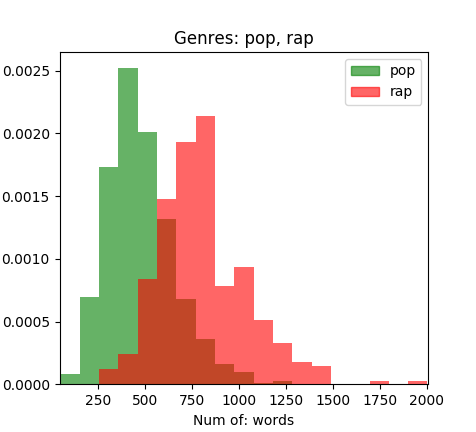
\includegraphics[width=\textwidth]{res/words-pop_rap.png}
        \caption{Number of words in pop and rap}
    \end{subfigure}
    ~ % spacing
    \begin{subfigure}[b]{0.48\textwidth}
        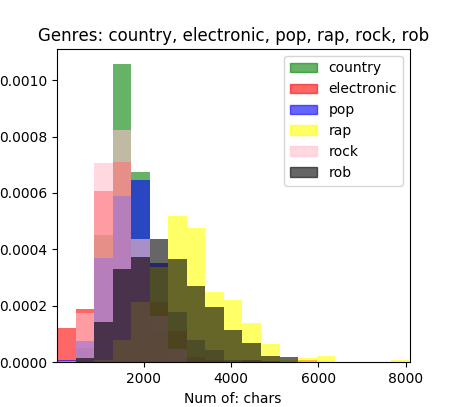
\includegraphics[width=\textwidth]{res/chars-country_electronic_pop_rap_rock_rob.png}
        \caption{Number of characters in all genres}
    \end{subfigure}
    \caption{Histograms over length of lyrics by genres}
    \label{fig:words}
\end{figure}

\subsection{Options}
To run and use the system several options were added:

\begin{itemize}
    \item {\textbf{Genres} - Default was to use all genres but could be changed to any genres provided in the project file.
    When certain features were tested it were only relevant to have a few number of genres.}
    \item {\textbf{Iterations} - During a test, the data was shuffled and then split up in training and test.
    Between different runs the result can differ so to get a reliable result the test needed to be run a number of times.
    The number of iterations were determined by this option.}
    \item {\textbf{Split} - In the baseline system the default value to split training and test data was 70\% and 30\% respectively.
    This can be changed with this parameter.}
    \item {\textbf{Count} - Default were to use all tracks in each genre.
    With this option the number of tracks in each genre were limited to the provided argument.
    This made testing of the model quicker.}
    \item {\textbf{Show features} - Provided with a value n. Shows the n most informative features in the model.}
    \item {\textbf{Statistics} - Show precision, recall and f-measure for each genre in the model.}
\end{itemize}

\subsection{Code}
During this project effort was made in making a good and usable system, for both scraping, use different features and run multiple tests.
The code can be found at GitHub. \cite{github}
Documentation on how to retrieve the corpus and run the system can be found in the repository's ``README''.

\section{Results}
The results will focus mainly on comparing two different genres or comparing all genres.
For all tests the split in training and test is 70\% and 30\% respectively.
If not stated differently, all tests have been running for 5 iterations.
All other arguments use the default values.
Between different tests the random seed was reset which makes the results reproducible.
Results will be presented for each feature explained in section \ref{sec:feat}.

Performance for the baseline system is shown in table \ref{tab:res-baseline}.
The 10 most informative features when comparing pop and rap are listed in table \ref{tab:num-feat} together with the ratio rap to pop.

\begin{table}[h]
\begin{center}
    \begin{tabular}{| l | r |}
        \hline
        Genres & Accuracy \\
        \hline
        all 6 genres & 53.20 \% \\
        pop and rap & 93.22 \% \\
        \hline
    \end{tabular}
    \caption{Accuracy of baseline system}
    \label{tab:res-baseline}
\end{center}
\end{table}


\begin{table}[h]
\begin{center}
    \begin{tabular}{| r | l | r |}
        \hline
        Number  & Unigram   & Ratio (rap:pop)   \\ \hline
        1       & Fuck      & 66:1              \\ \hline
        2       & bitches   & 59:1              \\ \hline
        3       & nigga     & 44:1              \\ \hline
        4       & niggas    & 41:1              \\ \hline
        5       & bitch     & 39:1              \\ \hline
        6       & rich      & 38:1              \\ \hline
        7       & fucked    & 36:1              \\ \hline
        8       & shit      & 31:1              \\ \hline
        9       & ho        & 29:1              \\ \hline
        10      & Nigga     & 29:1              \\ \hline
    \end{tabular}
    \caption{Most informative unigrams, pop and rap}
    \label{tab:num-feat}
\end{center}
\end{table}

\subsection{Unigrams}
\label{sec:unigrams}
The threshold value for the unigrams are examined for a number of values are shown in table \ref{tab:res-uni}.
The genres pop and rap are examined as well as all genres.
When using few features, stop words can result in a large difference. Therefore, each test was run twice, one normal and one without stop words.

\begin{table}[h]
\begin{center}
    \begin{tabular}{| r | r | r | r |}
        \hline
        \# of features  & Accuracy & Ignore stop words  & Time (seconds) \\
        \hline
        pop and rap     &          &            &       \\ \hline
        10              & 70.75 \% & 79.09 \%   & 1.4   \\
        50              & 84.43 \% & 85.99 \%   & 2.1   \\
        100             & 87.95 \% & 91.21 \%   & 1.8   \\
        500             & 91.99 \% & 92.77 \%   & 4.0   \\
        1000            & 92.25 \% & 92.77 \%   & 8.6   \\
        2500 (default)  & 93.22 \% & 93.09 \%   & 14.4  \\
        10000           & 92.51 \% & 91.73 \%   & 64.7  \\
        \hline
        all genres      &          &            &       \\ \hline
        10              & 33.82 \% & 36.37 \%   & 4.1   \\
        50              & 42.59 \% & 43.92 \%   & 5.3   \\
        100             & 46.24 \% & 46.49 \%   & 7.0   \\
        500             & 50.31 \% & 51.02 \%   & 18.3  \\
        1000            & 52.20 \% & 52.47 \%   & 33.7  \\
        2500 (default)  & 53.20 \% & 52.35 \%   & 74.3  \\
        10000           & 54.16 \% & 52.49 \%   & 277.7 \\
        \hline
    \end{tabular}
    \caption{Accuracy for unigrams thresholds, normal and ignoring stop words}
    \label{tab:res-uni}
\end{center}
\end{table}

\subsection{N-grams}
The different n-grams are examined individually, without unigrams and together with each other.
For all tests the threshold values are as defined in section \ref{sec:feat}: unigram 2500, bigram 2000, trigram 3000 and 1000 for four-gram and 1000 for five-gram.
As before, pop and rap are evaluated together with all genres.
The tests are shown in table \ref{tab:res-ngram}.
The first line is the baseline system, every test that performs better than that is marked green.

\begin{table}[H]
\begin{center}
    \begin{tabular}{| r | r | r | r | r | r | r |}
        \hline
        Uni & Bi & Tri & Four & Five & Accuracy (pop rap) & Accuracy (all) \\
        \hline
        % Unigram
        1 &   &   &   &   & 93.22 \% & 53.20 \% \\ \hline
        % Bigram
          & 1 &   &   &   &  92.44 \% & 47.76 \% \\ \hline
        1 & 1 &   &   &   &  93.09 \% & \cellcolor{Green} 54.16 \% \\ \hline
        % Trigram
          &   & 1 &   &   &  81.24 \% & 38.02 \% \\ \hline
        1 &   & 1 &   &   &  93.09 \% & \cellcolor{Green} 53.59 \% \\ \hline
        1 & 1 & 1 &   &   &  92.77 \% & \cellcolor{Green} 53.49 \% \\ \hline
        % Fourgram
          &   &   & 1 &   &  70.75 \% & 29.96 \% \\ \hline
        1 &   &   & 1 &   &  93.09 \% & \cellcolor{Green}54.25 \% \\ \hline
        1 & 1 & 1 & 1 &   &  92.83 \% & \cellcolor{Green}53.27 \% \\ \hline
        % Five-gram
          &   &   &   & 1 &  69.84 \% & 23.90 \% \\ \hline
        1 &   &   &   & 1 &  93.03 \% & \cellcolor{Green} 54.10 \% \\ \hline
        1 & 1 & 1 & 1 & 1 &  92.77 \% & 52.88 \% \\ \hline
    \end{tabular}
    \caption{Accuracy n-grams}
    \label{tab:res-ngram}
\end{center}
\end{table}

\subsection{Meta data}
The accuracy when adding the feature meta data is shown in table \ref{tab:res-meta}.
%Different tests are made with varying genres.
The accuracy is calculated by using the baseline system and then adding the feature.

\begin{table}[h]
\begin{center}
    \begin{tabular}{| r | r | r |}
        \hline
        Genres & Normal & Meta Data \\
        \hline
        all genres & 53.20 \% & 54.49 \% \\

        pop, rap & 93.22 \% & 93.29 \% \\

        country, rap & 97.05 \% & 97.41 \% \\

        electronic, rock & 75.47 \% & 77.53 \% \\

        electronic, r\&b & 82.15 \% & 82.20 \% \\
        \hline
    \end{tabular}
    \caption{Accuracy for meta data}
    \label{tab:res-meta}
\end{center}
\end{table}

\subsection{Word editing}
The three different word types are tested on all genres and on the genres pop and rap.
Results from the word editing are found in table \ref{tab:res-words}.

\begin{table}[h]
\begin{center}
    \begin{tabular}{| l | l | l | r | r | }
        \hline
        Stop words & Tokenize & Stem & Accuracy (pop rap) & Accuracy (all) \\
        \hline
          &   &   & 93.22 \% & 53.20 \% \\ \hline
        1 &   &   & 93.09 \% & 52.35 \% \\ \hline
          & 1 &   & 93.09 \% & 51.90 \% \\ \hline
          &   & 1 & 93.22 \% & 52.59 \% \\ \hline
        1 & 1 &   & 93.22 \% & 51.57 \% \\ \hline
        1 &   & 1 & 93.09 \% & 52.76 \% \\ \hline
          & 1 & 1 & 93.42 \% & 51.76 \% \\ \hline
        1 & 1 & 1 & 93.22 \% & 53.20 \% \\ \hline
    \end{tabular}
    \caption{Accuracy for word features}
    \label{tab:res-words}
\end{center}
\end{table}

\subsection{Length of lyrics}
The result regarding the three different features about the length of the lyrics is shown in table \ref{tab:res-lengths}.

\begin{table}[h]
\begin{center}
    \begin{tabular}{| l | l | l | r | r |}
        \hline
        Genres & Type (\# of)& Threshold & Accuracy (normal) & Accuracy (feature) \\
        \hline
        all genres      & characters    & 2000 & 53.20 \% & 53.20 \% \\ \hline
        electronic, pop & characters    & 2000 & 76.32 \% & 76.32 \% \\ \hline
        all genres            & words         & 600  & 53.20 \% & 53.25 \% \\ \hline
        country, rap    & words         & 600  & 97.05 \% & 97.32 \% \\ \hline
        all genres          & unique words  & 100  & 53.20 \% & 53.18 \% \\ \hline
        rock, r\&b      & unique words  & 100  & 88.57 \% & 88.70 \% \\ \hline
    \end{tabular}
    \caption{Accuracy for normal model and with feature added}
    \label{tab:res-lengths}
\end{center}
\end{table}

\subsection{Statistics}
For all tests the accuracy have been the measure of choice.
The precision, recall and f-measure for 5 tests are shown in table \ref{tab:res-stats1}.
These tests have been running for 1 iteration each.

\begin{table}[h]
\begin{center}
    \begin{tabular}{| r | l | r | r | r | r |}
        \hline
        Test & Genre & Accuracy & Precision & Recall & F-measure \\
        \hline
        1   & pop           & 93.16\%   & 95.77 \%  & 94.44 \%  & 95.10 \%  \\ \hline
        1   & rap           & 93.16\%   & 87.23 \%  & 90.11 \%  & 88.65 \%  \\ \hline
            &               &           &           &           &           \\ \hline
        2   & country       & 95.98\%   & 93.23 \%  & 100.00\%  & 96.50 \%  \\ \hline
        2   & rap           & 95.98\%   & 100.00\%  & 91.00 \%  & 95.29 \%  \\ \hline
            &               &           &           &           &           \\ \hline
        3   & pop           & 70.31\%   & 77.33 \%  & 63.03 \%  & 69.45 \%  \\ \hline
        3   & rock          & 70.31\%   & 64.86 \%  & 78.69 \%  & 71.11 \%  \\ \hline
            &               &           &           &           &           \\ \hline
        4   & rap           & 96.44\%   & 96.13 \%  & 98.31 \%  & 97.21 \%  \\ \hline
        4   & rock          & 96.44\%   & 97.00 \%  & 93.27 \%  & 95.10 \%  \\ \hline
            &               &           &           &           &           \\ \hline
        5   & country       & 53.98\%   & 82.57\%   & 77.59\%   & 80.00 \%  \\ \hline
        5   & electronic    & 53.98\%   & 49.23\%   & 50.79\%   & 50.00 \%  \\ \hline
        5   & pop           & 53.98\%   & 42.98\%   & 47.49\%   & 45.12 \%  \\ \hline
        5   & rap           & 53.98\%   & 54.96\%   & 67.92\%   & 60.76 \%  \\ \hline
        5   & rock          & 53.98\%   & 54.23\%   & 59.89\%   & 56.92 \%  \\ \hline
        5   & rob           & 53.98\%   & 53.89\%   & 38.96\%   & 45.23 \%  \\ \hline
    \end{tabular}
    \caption{Accuracy, precision, recall and f-measure for 5 different tests}
    \label{tab:res-stats1}
\end{center}
\end{table}

\pagebreak
\section{Discussion}
The results of the baseline system are found in table \ref{tab:res-baseline}.
Using all genres, the baseline system have the accuracy $53.20 \%$.
The data set used in this project is new, therefore the results can not be compared to results in other articles.
By only guessing the genre of a track, the accuracy would be $16.67 \%$ when choosing between 6 genres.
Compared to guessing, the baseline system seems to perform alright.

The two genres I was most interested in was pop and rap.
The classifier performs well to make a difference between the two genres, with an accuracy of $93.22 \%$.
Rap tends to contain more curses and bad language in general compared to pop.
Out of the 10 most informative features, 9 are curse words with 3 of them variations of the word ``nigga''.
% When writing a rap track, don't be afraid to curse.

\subsection{Unigrams}
The results for the unigrams are found in table \ref{tab:res-uni}.
For all number of features up to the default value of 2500, both tests performs better when removing the stop words.
Therefore, it is necessary to remove stop words when using few features.

With all genres, 100 features and removed stop words, the accuracy is $46.49\%$ and the execution time is 7 seconds.
The baseline system uses 2500 features, have an accuracy of $53.20\%$ and have an execution time of 74.3 seconds.
Taking the model's complexity into consideration the model performs really well with few features.

\subsection{N-grams}
When analyzing the n-grams the most information is found in the unigrams, as shown in table \ref{tab:res-ngram}.
With only rap and pop, the baseline system perform better than all other combinations.

For the tests with all genres, the n-gram features performs better.
No n-gram alone performs better than the n-gram together with unigrams.
However, all additions of a n-gram (except the last test with all n-grams added) improves the accuracy.
I realized that the four-grams and five-grams quickly became uninformative because they often consists of repetitions of words, for example ``la, la, la, la, la''.
With long n-grams it is hard to match anything else than that exact track it appears in, meaning the performance for them is low.
For example, five-grams alone have the accuracy of only $23.90 \%$.

\subsection{Meta data}
The feature meta data made an improvement in all tests, as shown in table \ref{tab:res-meta}.
The increased accuracy was not of great magnitude but still an increase.
For example, the test with all genres made an increase in accuracy from $53.20\%$ to $54.49 \%$.
Meta data is a feature that looks on the structure of the song.
This result indicates that the structure of a song is important when classifying genres.

\subsection{Word editing}
For the two genres pop and rap, adding the word features did not make a big impact on the accuracy.
As seen in table \ref{tab:res-words}, 3 of the tests had the same accuracy, 3 performed slightly worse and 1 performed slightly better.
In the tests with all genres, no test performed better than the baseline system.
Removing stop words did make a difference when 2500 unigram features were used.
More interesting results are found when removing stop words using fewer unigram features, discussed previously and shown in table \ref{tab:res-uni}.

These results show that the word editing features are not that important for the classifier.
Even if stop words contain a lot of noise, they still contain information about the genre.
With so many as 2500 unigram features there is no need for a stemmer, which destroys information.

\subsection{Length of lyrics}
Adding features about the length of the lyrics did not change the accuracy of the baseline system very much, as shown in table \ref{tab:res-lengths}.
As shown in figure \ref{fig:words}b, there is hard to differentiate between several genres.
Therefore, with too many genres, these features do not seem to be useful.
Instead, it is necessary to compare only a few genres when using features about the length of the lyrics.
Pop and rap have differences in lengths, as shown in figure \ref{fig:words}a.
Between these genres it is a clear distinction.
Also, a significant difference is found between country and rap, which give an increase in accuracy, from $97.05\%$ to $97.32\%$, as seen in table \ref{tab:res-lengths}.

\subsection{Statistics}
The accuracy is easy to compare to each other but does not tell how well the classifier performs on the individual genres.
For this reason the precision, recall and f-measure were calculated for a number of tests, which are shown in table \ref{tab:res-stats1}.

Looking at the other performance measures, the tests were included for different reasons.
During the project the genres pop and rap have been the main focus, the classifier performs better to classify pop than rap.
For country and rap, the classifier succeeds to get $100\%$ in rap precision and $100\%$ in country recall which is quite interesting.
Pop and rock are hard for the classifier to differentiate between, with an accuracy of $70.31\%$, which suggests that the lyrics in them are quite similar.
In contrast, rap and rock have the highest accuracy with $96.44\% $.

\section{Conclusion}
In the project, I tried to find features that could improve the performance of the Naive Bayes classifier.
I succeeded in finding features that made a positive impact on the performance.
The results were not groundbreaking but it was interesting to see that features like the structure of the track (meta data), and the different n-grams made a difference when classifying the tracks.

I learned a lot from this project.
A huge amount of time was invested in creating the corpus.
Using a previously created corpus would have saved much time.
If I would do a similar project again, I would most likely choose a project with an existing corpus, for example tweets or news articles.

When exploring all features many tests were needed, therefore I built a system for analyzing the tests.
This initially took a lot of time, but in the end, I specified the tests I wanted for the report and executed them in a big test run.
The tests are specified in the Python file ``src/tests.py'' in the GitHub repository.

\pagebreak
\bibliographystyle{ieeetr}
\bibliography{res/classy}

\end{document}

